% Draft v0.1 (2026-11-15). Every number comes from analysis/paper_tables.py (numbers.tex, tables/,
% figures/) or analysis/confirm_test.py. Do not type numbers by hand.
\documentclass[11pt]{article}
\usepackage[margin=1in]{geometry}
\usepackage[T1]{fontenc}
\usepackage{lmodern,amsmath,amssymb,booktabs,graphicx,xcolor}
\usepackage[numbers,sort&compress]{natbib}
\usepackage[colorlinks=true,linkcolor=blue!50!black,citecolor=blue!50!black,urlcolor=blue!50!black]{hyperref}
\newcommand{\nExplore}{25}
\newcommand{\nConfirm}{14}
\newcommand{\nTotal}{39}
\newcommand{\rhoExplore}{+0.95}
\newcommand{\rhoConfirm}{+0.95}
\newcommand{\pConfirm}{1.4\times10^{-7}}
\newcommand{\tsGainConfirm}{+1.02}
\newcommand{\tostP}{0.53}
\newcommand{\worseNoneExplore}{13}
\newcommand{\worseNoneConfirm}{4}
\newcommand{\worseTsExplore}{25}
\newcommand{\worseTsConfirm}{14}
\newcommand{\oracleEceRel}{83}
\newcommand{\oracleAurocGain}{+3.04}
\newcommand{\shareER}{61--92}
\newcommand{\shareDERpp}{22--64}
\newcommand{\shareMIR}{70--76}
\newcommand{\shareiCaRL}{10--13}
\newcommand{\confoundOld}{+14.9}
\newcommand{\confoundAll}{+2.6}
\newcommand{\rhoWithinER}{+0.89}
\newcommand{\rhoWithinDERpp}{+0.91}
\newcommand{\rhoChance}{+0.95}
\newcommand{\rhoAURC}{+0.91}
\newcommand{\oldnewCorr}{+1.00}
\newcommand{\oldnewWorseTs}{39}
\newcommand{\heldERmsp}{73.1}
\newcommand{\heldERpred}{87.7}
\newcommand{\heldERtrue}{54.7}
\newcommand{\heldEReceTs}{4.8}
\newcommand{\heldEReceTrue}{30.5}
\newcommand{\heldEReceTp}{7.3}
\newcommand{\heldDmsp}{78.4}
\newcommand{\heldDpred}{83.0}
\newcommand{\heldDeceTs}{5.6}
\newcommand{\heldDeceTp}{3.7}
\newcommand{\heldERtold}{5.2}

\newcommand{\taskts}{task-TS}

\title{Recency Bias Decides When Task-Aware Calibration Helps a Continual Learner Detect Its Own Errors:\\
A Pre-registered Study in Class-Incremental Learning}
\author{Anonymous}
\date{}

\begin{document}
\maketitle

\begin{abstract}
Recent post-hoc calibration methods for class-incremental learning (CIL) fit temperatures per task
on the replay buffer and are evaluated by calibration error alone. We ask whether such calibrators
also help a model \emph{detect its own errors}, the property selective prediction depends on. On
seq-CIFAR-10/100 with ER, DER++, MIR and iCaRL (\nTotal{} runs), we report three findings. (i)~A
methodological pitfall: the common old-class-only error-detection AUROC is confounded for any score
that depends on the predicted task, inflating the apparent gain of task-aware temperature scaling
from \confoundAll{} to \confoundOld{} AUROC points on average. (ii)~Whether task-aware temperature
scaling helps or hurts failure detection is governed by recency bias, the share of old-class errors
that are predicted as a current-task class. This was found on \nExplore{} exploratory runs
(Spearman $\rho=\rhoExplore$) and then confirmed under a rule committed before \nConfirm{} new runs
with unseen seeds and two unseen methods ($\rho=\rhoConfirm$, $p=\pConfirm$). (iii)~The mechanism:
the buffer is memorised (about 100\,\% accuracy), so the fitted old-task temperatures collapse to
about $0.1$ while the current-task temperature stays near the global one. Task-aware scaling then
behaves like a trivial rule that distrusts current-task predictions. Its failure-detection gain
tracks that rule's gain almost exactly (correlation $\geq 0.98$ for ER, MIR and DER++), and it
calibrates worse than a single global temperature in every one of our \nTotal{} runs. Three further
pre-registered claims about global and oracle temperatures were not confirmed, and we report them
as such.
\end{abstract}

\section{Introduction}
A continual learner that forgets should at least know when it is wrong. In class-incremental
learning (CIL)~\cite{vandeven2022three,masana2022survey}, a single classifier must cover all classes
seen so far without task labels at test time. Models are known to be miscalibrated after
learning several tasks~\cite{li2024calibration}, and recent work proposes post-hoc fixes:
temperature scaling with perturbed exemplars (T-CIL~\cite{hwang2025tcil}), distance-aware
temperatures (DATS~\cite{dats2025}) and multi-temperature schemes~\cite{mtcc2026}. These methods
are evaluated by calibration metrics such as ECE. However, calibration and \emph{failure
detection}, i.e.\ ranking a model's errors below its correct predictions, are different
properties~\cite{jaeger2023call,zhu2022rethinking}, and the second is what selective prediction
and deferral to a human need~\cite{geifman2017selective}.

We study what post-hoc temperature calibrators do to failure detection in CIL, using only saved
logits, so every analysis runs on a CPU. The study has two stages. We first analysed
\nExplore{} runs and found that the original hypothesis, that calibrators do not help detection,
was not supported in its pre-registered form (Section~\ref{sec:design}). We then wrote down four
specific claims suggested by that data and tested them on \nConfirm{} new runs that nobody had
looked at, under a decision rule committed to version control beforehand.

\paragraph{Contributions.}
\begin{itemize}
\item \textbf{A measurement pitfall.} Restricting error-detection AUROC to test samples whose
  \emph{true} class is old leaks label information into any score that depends on the
  \emph{predicted} task, because among true-old samples every current-task prediction is an error.
  We show that this inflates gains by a large factor and recommend all-class AUROC for such scores
  (Section~\ref{sec:pitfall}).
\item \textbf{A confirmed predictor.} The failure-detection gain of task-aware temperature scaling
  is predicted by the recency share of old-class errors. This holds on unseen seeds and on two
  methods not used to form the hypothesis (MIR and iCaRL), with $\rho=\rhoConfirm$
  (Section~\ref{sec:recency}).
\item \textbf{A mechanism.} Per-task temperatures fitted on a memorised buffer degenerate, so
  task-aware scaling reduces to ``distrust current-task predictions''. This explains when it helps,
  when it hurts, and why it calibrates worse than one global temperature (Section~\ref{sec:mech}).
\item \textbf{Negative and null results reported in full}, including three pre-registered claims
  that were not confirmed (Section~\ref{sec:null}).
\end{itemize}

\section{Related work}
\paragraph{Class-incremental learning.} Replay methods such as ER~\cite{chaudhry2019tiny},
DER++~\cite{buzzega2020dark}, MIR~\cite{aljundi2019mir} and iCaRL~\cite{rebuffi2017icarl} keep a
small memory of past data. CIL models are biased towards the most recent classes; this
\emph{recency} or task-recency bias is well documented and motivates output-layer corrections such
as BiC~\cite{wu2019bic}, LUCIR~\cite{hou2019lucir} and separated softmax~\cite{ahn2021ssil}. We
measure this bias among the model's errors and use it to explain the behaviour of calibrators,
rather than correcting it.

\paragraph{Calibration in continual learning.} \citet{li2024calibration} showed that continual
learners are poorly calibrated. T-CIL~\cite{hwang2025tcil}, DATS~\cite{dats2025} and
MT-CC~\cite{mtcc2026} propose temperature-based calibrators for CIL and report calibration metrics.
Our task-aware calibrators are deliberately simple versions of this family (one temperature per
task, or per old/new group, assigned by the predicted task). We do not claim to reproduce those
methods (Section~\ref{sec:limits}).

\paragraph{Failure detection.} Maximum softmax probability (MSP)~\cite{hendrycks2017baseline} is
a strong baseline for misclassification detection. \citet{jaeger2023call} argue that failure
detection should be evaluated by ranking metrics such as AUROC and AURC rather than calibration
error. \citet{zhu2022rethinking} show that popular calibration methods can harm failure prediction.
We bring this view to CIL, where the old/new class structure creates a pitfall of its own.

\section{Setup}\label{sec:setup}
\paragraph{Benchmarks and training.} seq-CIFAR-10 (5 tasks $\times$ 2 classes) and seq-CIFAR-100
(10 tasks $\times$ 10 classes)~\cite{krizhevsky2009learning}. We use a reduced ResNet-18, SGD,
batch size 32 and 50 epochs per task, following the DER protocol~\cite{buzzega2020dark}, with
per-method hyper-parameters from the public Mammoth configurations and mixed-precision training.
Each task's training set is split 90/10 into training and validation; test sets are never used for
fitting. Buffer sizes are 500 and 2000. Our DER++ reaches $71.2\pm3.4$ final accuracy on
seq-CIFAR-10 (published: $72.7\pm1.4$~\cite{buzzega2020dark}). Final accuracies on seq-CIFAR-100
are listed in Appendix~\ref{app:acc}.

\paragraph{Scores and calibrators.} All scores are computed from the logits after the last task.
Temperatures never change the argmax, so accuracy is identical across calibrators.
\begin{itemize}
\item \textbf{MSP}: maximum softmax probability, no calibration.
\item \textbf{TS}: one global temperature minimising NLL~\cite{guo2017calibration}.
\item \textbf{\taskts}: one temperature per task, fitted on that task's calibration items. A test
  input uses the temperature of the task its \emph{predicted} class belongs to. A group with fewer
  than 20 items falls back to the global temperature.
\item \textbf{Oracle TS}: one temperature fitted on the evaluated old-class test data itself. This
  is not a method but an upper bound for any single temperature.
\end{itemize}
\paragraph{Legal calibration set.} At the end of training a CIL method may keep only its buffer and
the current task's validation split. All non-oracle calibrators are fitted on exactly this set. For
iCaRL, whose classifier is nearest-mean-of-exemplars, we use the logits
$-\lVert f(x)-\mu_c\rVert^2/\tau$ with $\tau=0.1$ on normalised features.

\paragraph{Metrics.} \textbf{ECE} with 15 equal-width bins; \textbf{error-detection AUROC}, the
probability that a correct prediction receives a higher score than an error; both in percent, on
\emph{all seen classes} unless stated otherwise. \textbf{Recency share}: among test samples of old
classes that are misclassified, the percentage predicted as a class of the current (last) task. If
errors were spread uniformly over the other classes, this would be 22\,\% on seq-CIFAR-10 and 10\,\%
on seq-CIFAR-100.

\section{Study design}\label{sec:design}
\paragraph{Stage 1: exploratory.} A first rule, committed before the analysis, stated that
calibrators improve calibration but not old-class failure detection. It was \emph{not supported}:
task-aware calibrators appeared to raise old-class AUROC by about 15 points. Inspecting why led to
the pitfall in Section~\ref{sec:pitfall} and to the recency hypothesis. These \nExplore{} runs (ER
and DER++; seq-CIFAR-10 at buffer 500 in three training variants, seq-CIFAR-100 at buffers 500 and
2000; 2--3 seeds per cell) are therefore exploratory, and are shown in
Appendix~\ref{app:explore}.

\paragraph{Stage 2: confirmatory.} Before any new run existed, we committed a test script with four
claims and their decision rules. It uses only \nConfirm{} new runs on seq-CIFAR-100: ER and DER++
with unseen seeds (3, 4) at buffers 500 and 2000, plus MIR and iCaRL (never analysed before) at
buffer 2000 with seeds 0--2. No pooling with stage-1 runs.
\begin{itemize}
\item[C1] Global TS changes AUROC$_\mathrm{all}$ by less than $\pm1$ point (equivalence by two
  one-sided $t$-tests, each $p<0.05$).
\item[C2] \taskts{} raises ECE$_\mathrm{all}$ above MSP in $\geq75\,\%$ of runs (sign test,
  $p<0.05$).
\item[C3] The recency share and the \taskts{} gain in AUROC$_\mathrm{all}$ are positively rank
  correlated (Spearman, one-sided $p<0.05$).
\item[C4] Oracle TS lowers ECE$_\mathrm{old}$ by $\geq50\,\%$ on average while raising
  AUROC$_\mathrm{old}$ by $<3$ points.
\end{itemize}
Analyses in Section~\ref{sec:mech} were done after the confirmation and are labelled post hoc.

\section{Results}
\subsection{Old-class-only AUROC is confounded for predicted-task scores}\label{sec:pitfall}
CIL papers often report uncertainty on old classes only, since forgetting happens there.
Restricting the evaluation to samples whose true class is old is harmless for a score that ignores
the predicted task, such as MSP or global TS. It is not harmless for \taskts: conditioned on a true
old class, \emph{every} prediction in the current task is an error, so any score that is lower for
current-task predictions becomes an error detector that cannot be used at deployment, where the
true class is unknown. On the exploratory runs, \taskts{} gains \confoundOld{} AUROC points under
the old-class-only metric but only \confoundAll{} points under the all-class metric. We therefore
evaluate predicted-task scores on all seen classes, and use old-class AUROC only for
task-independent scores (Table~\ref{tab:oracle}).

\subsection{Recency bias predicts the effect of task-aware calibration (confirmed)}\label{sec:recency}
Table~\ref{tab:confirm} shows the confirmatory runs and Figure~\ref{fig:recency} shows all runs.
The effect of \taskts{} on failure detection ranges from strongly negative to strongly positive.
Its sign and size follow the recency share: ER and MIR send most old-class errors to the current
task (recency share \shareER{}\,\% and \shareMIR{}\,\%) and, in the confirmatory runs, gain 13--22 AUROC
points. iCaRL, whose nearest-mean classifier does not use the biased output layer, has a share of \shareiCaRL{}\,\%, barely
above the uniform 10\,\%, and gains about 1 point. DER++ lies in between, and on seq-CIFAR-10 it
loses up to 20 points. On the confirmatory runs, Spearman $\rho=\rhoConfirm$ ($p=\pConfirm$);
\textbf{C3 is confirmed}. Two of the four confirmatory methods were not used to form the
hypothesis.

\begin{table*}[t]\centering\small
\caption{Confirmatory runs (never analysed before the rule was committed), state after the last task, all seen classes. Recency share: old-class errors predicted as a current-task class (uniform errors: 10\%). Mean{\scriptsize$\pm$sd} over seeds.}\label{tab:confirm}
\resizebox{\linewidth}{!}{\begin{tabular}{lllc c ccc ccc}\toprule
 & & & & recency & \multicolumn{3}{c}{AUROC$_\mathrm{all}$ ($\uparrow$)} & \multicolumn{3}{c}{ECE$_\mathrm{all}$ ($\downarrow$)}\\
\cmidrule(lr){6-8}\cmidrule(lr){9-11}
benchmark & method & $|M|$ & $n$ & share (\%) & MSP & TS & task-TS & MSP & TS & task-TS\\\midrule
S-CIFAR-100 & ER & 500 & 2 & 90.0{\scriptsize$\pm$2.6} & 66.8{\scriptsize$\pm$0.1} & 68.3{\scriptsize$\pm$0.1} & 88.7{\scriptsize$\pm$0.2} & 63.3{\scriptsize$\pm$2.9} & 48.0{\scriptsize$\pm$5.3} & 53.7{\scriptsize$\pm$3.8}\\
S-CIFAR-100 & ER & 2000 & 2 & 75.2{\scriptsize$\pm$5.4} & 74.2{\scriptsize$\pm$0.6} & 75.6{\scriptsize$\pm$0.5} & 87.3{\scriptsize$\pm$1.3} & 45.7{\scriptsize$\pm$1.2} & 34.2{\scriptsize$\pm$2.5} & 43.1{\scriptsize$\pm$0.8}\\
S-CIFAR-100 & DER++ & 500 & 2 & 60.0{\scriptsize$\pm$3.5} & 74.6{\scriptsize$\pm$0.5} & 74.5{\scriptsize$\pm$0.6} & 81.9{\scriptsize$\pm$0.7} & 19.3{\scriptsize$\pm$0.5} & 28.3{\scriptsize$\pm$2.3} & 45.7{\scriptsize$\pm$1.5}\\
S-CIFAR-100 & DER++ & 2000 & 2 & 52.5{\scriptsize$\pm$11.7} & 79.0{\scriptsize$\pm$3.2} & 79.1{\scriptsize$\pm$3.2} & 81.1{\scriptsize$\pm$0.8} & 20.6{\scriptsize$\pm$5.6} & 18.5{\scriptsize$\pm$2.3} & 34.8{\scriptsize$\pm$0.1}\\
S-CIFAR-100 & iCaRL & 2000 & 3 & 11.5{\scriptsize$\pm$1.3} & 75.5{\scriptsize$\pm$0.3} & 77.2{\scriptsize$\pm$0.7} & 76.7{\scriptsize$\pm$0.4} & 24.0{\scriptsize$\pm$0.8} & 8.8{\scriptsize$\pm$0.6} & 11.9{\scriptsize$\pm$0.5}\\
S-CIFAR-100 & MIR & 2000 & 3 & 73.4{\scriptsize$\pm$2.7} & 74.0{\scriptsize$\pm$0.7} & 75.3{\scriptsize$\pm$0.8} & 86.8{\scriptsize$\pm$0.7} & 44.8{\scriptsize$\pm$1.2} & 32.1{\scriptsize$\pm$1.5} & 41.6{\scriptsize$\pm$1.1}\\
\bottomrule\end{tabular}}
\end{table*}


\begin{figure}[t]\centering
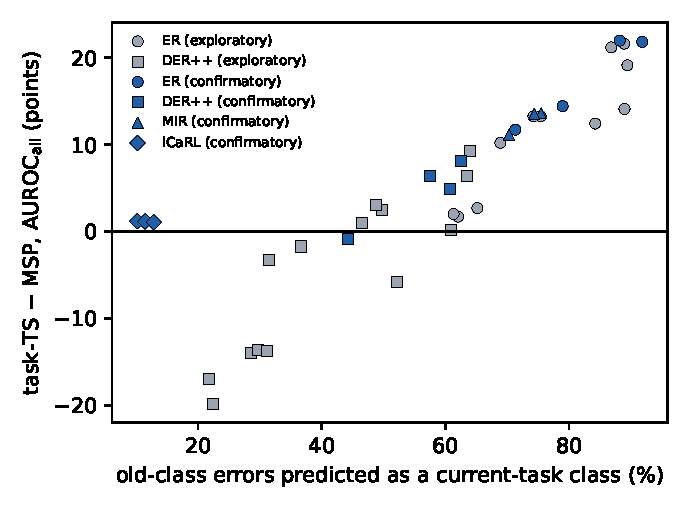
\includegraphics[width=0.62\linewidth]{figures/recency_gain}
\caption{Gain of \taskts{} over MSP in all-class failure-detection AUROC against the recency share
of old-class errors, one point per run. Grey: exploratory runs (used to form the hypothesis).
Blue: confirmatory runs (rule committed before they existed).}\label{fig:recency}
\end{figure}

\subsection{Why: per-task temperatures fitted on a memorised buffer degenerate (post hoc)}\label{sec:mech}
Table~\ref{tab:mech} shows the fitted temperatures. Replay buffers are trained on repeatedly, so
the model classifies them almost perfectly (99.9--100\,\% accuracy for ER, MIR and DER++). The NLL
on such items keeps falling as the temperature goes down, so old-task temperatures end near
$0.1$--$0.15$, while the current-task temperature, fitted on held-out validation data, stays close
to the global one. Under \taskts, every prediction that lands in an old task therefore gets a
confidence near 1, and the score mostly encodes \emph{which task was predicted}.

To test this reading we compare \taskts{} with a rule that uses no temperature at all: rank every
prediction in an old task above every prediction in the current task, and break ties by MSP. For
ER, MIR and DER++, the rule's AUROC is within about 1.4 points of \taskts{} on average, and their
gains over MSP correlate at $+0.98$ to $+1.00$ across runs. The rule helps exactly when errors sit in
the current task, which is what the recency share measures; this makes C3 a consequence of the
mechanism rather than a coincidence. iCaRL is the exception that fits the account: its exemplars
are not memorised under the nearest-mean classifier (63\,\% accuracy), its temperatures stay close
together, and \taskts{} behaves like global TS (only 3 runs, so we do not interpret the correlation
there).

The same mechanism hurts calibration. Old-task predictions become far too confident, and
\taskts{} has a higher ECE$_\mathrm{all}$ than global TS in \worseTsExplore/\nExplore{} exploratory
and \worseTsConfirm/\nConfirm{} confirmatory runs. This comparison was not pre-registered (see
C2 below).

\begin{table}[t]\centering\small
\caption{Why task-TS behaves as it does (post-hoc analysis over all 39 runs). Temperatures fitted on the legal calibration set; $T_\mathrm{old}$ is the mean over old tasks. \emph{Rule}: rank predictions in an old task above predictions in the current task, ties broken by MSP. Last column: Pearson correlation, over runs, of the AUROC$_\mathrm{all}$ gains of task-TS and of the rule.}\label{tab:mech}
\begin{tabular}{lc c ccc ccc c}\toprule
 & & buffer & \multicolumn{3}{c}{temperature} & \multicolumn{3}{c}{AUROC$_\mathrm{all}$} & \\
\cmidrule(lr){4-6}\cmidrule(lr){7-9}
method & $n$ & acc. (\%) & global & $T_\mathrm{old}$ & $T_\mathrm{cur}$ & MSP & task-TS & rule & corr.\\\midrule
ER & 15 & 100.0 & 2.02 & 0.15 & 2.15 & 73.1 & 86.5 & 86.8 & +1.00\\
MIR & 3 & 100.0 & 1.77 & 0.11 & 2.01 & 74.0 & 86.8 & 87.2 & +1.00\\
DER++ & 18 & 99.9 & 1.12 & 0.12 & 1.20 & 78.4 & 75.7 & 77.1 & +0.98\\
iCaRL & 3 & 63.0 & 0.43 & 0.38 & 0.54 & 75.5 & 76.7 & 71.2 & -0.83\\
\bottomrule\end{tabular}
\end{table}


\subsection{Pre-registered claims that were not confirmed}\label{sec:null}
\paragraph{C1 (global TS leaves failure detection unchanged): not confirmed.} The mean change was
\tsGainConfirm{} AUROC points (TOST $p=\tostP$). The effect is close to zero for DER++ and $+1.2$ to
$+1.9$ for ER, MIR and iCaRL. Global TS thus improves detection slightly, and our $\pm1$ margin was
too tight to claim equivalence.

\paragraph{C2 (task-TS worsens ECE over MSP in $\geq 75\,\%$ of runs): not confirmed.} Only
\worseNoneConfirm/\nConfirm{} runs. This claim rested on a counting error in our stage-1 notes: the
correct stage-1 count is \worseNoneExplore/\nExplore{}, not the 22/25 that we had recorded. The pattern is
method-dependent: for ER and MIR, uncalibrated ECE is so high (45--63) that even \taskts{} lowers
it, whereas for DER++ it rises. The robust statement is the comparison with global TS in
Section~\ref{sec:mech}, which needs its own confirmation.

\paragraph{C4 (oracle TS: large calibration gain, small detection gain): not confirmed.} An oracle
temperature lowered ECE$_\mathrm{old}$ by \oracleEceRel\,\% but raised AUROC$_\mathrm{old}$ by
\oracleAurocGain{} points, just above the 3-point threshold. Qualitatively, a single temperature
can remove most of the calibration error while changing the error ranking by only a few points
(Table~\ref{tab:oracle}), but the pre-registered criterion was missed.

\begin{table}[t]\centering\small
\caption{Old classes only, task-independent scores (where old-class AUROC is valid). Oracle TS is fitted on the evaluated old-class test data itself and is an upper bound for any single temperature. Mean over runs; relative ECE change is averaged per run.}\label{tab:oracle}
\begin{tabular}{lc ccc ccc}\toprule
 & & \multicolumn{3}{c}{ECE$_\mathrm{old}$} & \multicolumn{3}{c}{AUROC$_\mathrm{old}$}\\
\cmidrule(lr){3-5}\cmidrule(lr){6-8}
set & $n$ & MSP & TS & oracle TS & MSP & TS & oracle TS\\\midrule
exploratory & 25 & 33.4{\scriptsize$\pm$18.6} & 26.4{\scriptsize$\pm$13.2} & 5.8{\scriptsize$\pm$2.1} & 71.8{\scriptsize$\pm$7.9} & 72.4{\scriptsize$\pm$7.2} & 73.8{\scriptsize$\pm$5.9}\\
confirmatory & 14 & 39.1{\scriptsize$\pm$18.0} & 29.8{\scriptsize$\pm$14.9} & 5.2{\scriptsize$\pm$2.9} & 69.6{\scriptsize$\pm$8.6} & 70.8{\scriptsize$\pm$8.2} & 72.6{\scriptsize$\pm$6.4}\\
\bottomrule\end{tabular}
\end{table}


\section{Discussion}
\paragraph{What this means in practice.} A task-aware calibrator fitted on the replay buffer is
not a calibrator in the usual sense: its temperatures reflect how well the buffer was memorised,
not how reliable the model is on old classes. Its benefit for failure detection is real only when
the model's errors are dominated by recency bias, and a simple ``distrust the newest task'' rule
captures it. CIL calibration methods should therefore (a)~report failure-detection metrics on all
seen classes alongside ECE, (b)~compare against the predicted-task rule, and (c)~avoid fitting
per-task temperatures on memorised data, the problem T-CIL addresses with perturbed
exemplars~\cite{hwang2025tcil}.

\paragraph{Limitations.}\label{sec:limits} We evaluate simplified task-aware calibrators, not the
published T-CIL, DATS or MT-CC implementations, so our results bound what those methods do only to
the extent that they share the per-task temperature structure. Confirmation covers seq-CIFAR-100
only, with 2--3 seeds per cell; seq-CIFAR-10 and the training-variant runs are exploratory. The
recency share requires test labels and is a diagnostic, not a deployable score; whether a
label-free proxy (e.g.\ the fraction of predictions falling in the current task) works is open.
iCaRL's uncalibrated ECE depends on the arbitrary scale $\tau$ of its nearest-mean logits. The
mechanism analysis is post hoc. Finally, the backbone is a ResNet-18 trained from scratch;
pre-trained models may behave differently.

\section{Conclusion}
Whether task-aware temperature scaling helps a class-incremental learner detect its own errors is
decided by recency bias, a prediction we confirmed on unseen runs and methods. The reason is
simple: per-task temperatures fitted on a memorised buffer turn the calibrator into a
predicted-task indicator. We hope the pitfall, the predictor and the rule baseline make future CIL
calibration studies easier to interpret.

\paragraph{Reproducibility.} Code, configurations, per-run logs and metrics, the pre-registration
commits and the scripts that generate every number, table and figure in this paper are public
(link withheld for review). The confirmation rule was committed before the confirmatory runs were
started.

\bibliographystyle{plainnat}
\bibliography{refs}

\appendix
\section{Exploratory runs}\label{app:explore}
\begin{table*}[t]\centering\small
\caption{Exploratory runs (used to form the hypotheses), same quantities as Table~\ref{tab:confirm}. Uniform-error recency baseline: 22\% on S-CIFAR-10, 10\% on S-CIFAR-100.}\label{tab:explore}
\resizebox{\linewidth}{!}{\begin{tabular}{lllc c ccc ccc}\toprule
 & & & & recency & \multicolumn{3}{c}{AUROC$_\mathrm{all}$ ($\uparrow$)} & \multicolumn{3}{c}{ECE$_\mathrm{all}$ ($\downarrow$)}\\
\cmidrule(lr){6-8}\cmidrule(lr){9-11}
benchmark & method & $|M|$ & $n$ & share (\%) & MSP & TS & task-TS & MSP & TS & task-TS\\\midrule
S-CIFAR-10 & ER (lr decay) & 500 & 3 & 71.8{\scriptsize$\pm$15.0} & 78.2{\scriptsize$\pm$2.7} & 78.8{\scriptsize$\pm$2.8} & 84.4{\scriptsize$\pm$4.3} & 35.1{\scriptsize$\pm$5.0} & 27.2{\scriptsize$\pm$5.9} & 33.7{\scriptsize$\pm$4.1}\\
S-CIFAR-10 & ER (fp32) & 500 & 2 & 73.2{\scriptsize$\pm$15.7} & 77.6{\scriptsize$\pm$4.8} & 78.3{\scriptsize$\pm$5.0} & 84.7{\scriptsize$\pm$2.8} & 34.3{\scriptsize$\pm$8.2} & 26.5{\scriptsize$\pm$9.2} & 32.8{\scriptsize$\pm$6.9}\\
S-CIFAR-10 & DER++ & 500 & 3 & 34.8{\scriptsize$\pm$15.5} & 80.2{\scriptsize$\pm$2.1} & 80.2{\scriptsize$\pm$2.2} & 67.1{\scriptsize$\pm$5.6} & 16.9{\scriptsize$\pm$3.7} & 11.0{\scriptsize$\pm$2.7} & 23.6{\scriptsize$\pm$2.3}\\
S-CIFAR-10 & DER++ (lr decay) & 500 & 3 & 37.9{\scriptsize$\pm$20.5} & 79.8{\scriptsize$\pm$2.3} & 79.7{\scriptsize$\pm$2.5} & 69.6{\scriptsize$\pm$6.9} & 16.7{\scriptsize$\pm$4.1} & 12.1{\scriptsize$\pm$5.8} & 23.9{\scriptsize$\pm$2.5}\\
S-CIFAR-10 & DER++ (fp32) & 500 & 2 & 46.1{\scriptsize$\pm$24.7} & 76.5{\scriptsize$\pm$8.6} & 76.5{\scriptsize$\pm$8.7} & 72.7{\scriptsize$\pm$5.9} & 20.0{\scriptsize$\pm$10.9} & 11.1{\scriptsize$\pm$8.4} & 23.8{\scriptsize$\pm$4.6}\\
S-CIFAR-100 & ER & 500 & 3 & 88.4{\scriptsize$\pm$1.4} & 67.3{\scriptsize$\pm$1.5} & 69.0{\scriptsize$\pm$1.3} & 88.0{\scriptsize$\pm$0.2} & 62.4{\scriptsize$\pm$2.1} & 44.3{\scriptsize$\pm$1.7} & 50.6{\scriptsize$\pm$0.9}\\
S-CIFAR-100 & ER & 2000 & 3 & 72.9{\scriptsize$\pm$3.5} & 74.0{\scriptsize$\pm$1.0} & 75.2{\scriptsize$\pm$1.0} & 86.2{\scriptsize$\pm$0.8} & 45.1{\scriptsize$\pm$1.0} & 32.6{\scriptsize$\pm$1.0} & 42.2{\scriptsize$\pm$0.4}\\
S-CIFAR-100 & DER++ & 500 & 3 & 54.2{\scriptsize$\pm$8.5} & 75.8{\scriptsize$\pm$2.3} & 75.8{\scriptsize$\pm$2.3} & 80.8{\scriptsize$\pm$1.5} & 16.9{\scriptsize$\pm$3.1} & 23.8{\scriptsize$\pm$2.8} & 44.4{\scriptsize$\pm$0.3}\\
S-CIFAR-100 & DER++ & 2000 & 3 & 38.2{\scriptsize$\pm$7.6} & 81.0{\scriptsize$\pm$0.7} & 80.9{\scriptsize$\pm$0.7} & 79.6{\scriptsize$\pm$1.5} & 14.2{\scriptsize$\pm$2.0} & 14.8{\scriptsize$\pm$2.1} & 36.2{\scriptsize$\pm$0.6}\\
\bottomrule\end{tabular}}
\end{table*}


\section{Final accuracy}\label{app:acc}
Final average accuracy (\%) on seq-CIFAR-100, mean$\pm$sd over seeds: ER $21.6\pm1.8$ (buffer 500,
5 seeds) and $38.9\pm0.9$ (2000, 5 seeds); DER++ $36.7\pm1.2$ (500, 5 seeds) and $50.6\pm2.9$
(2000, 5 seeds); MIR $39.8\pm1.3$ and iCaRL $44.7\pm0.8$ (2000, 3 seeds). Source:
\texttt{tables/summary.md}.
% TODO: generate this paragraph from analysis/summarize.py instead of copying it.

\end{document}
